% Created by tikzDevice version 0.12.6 on 2024-06-15 18:34:42
% !TEX encoding = UTF-8 Unicode
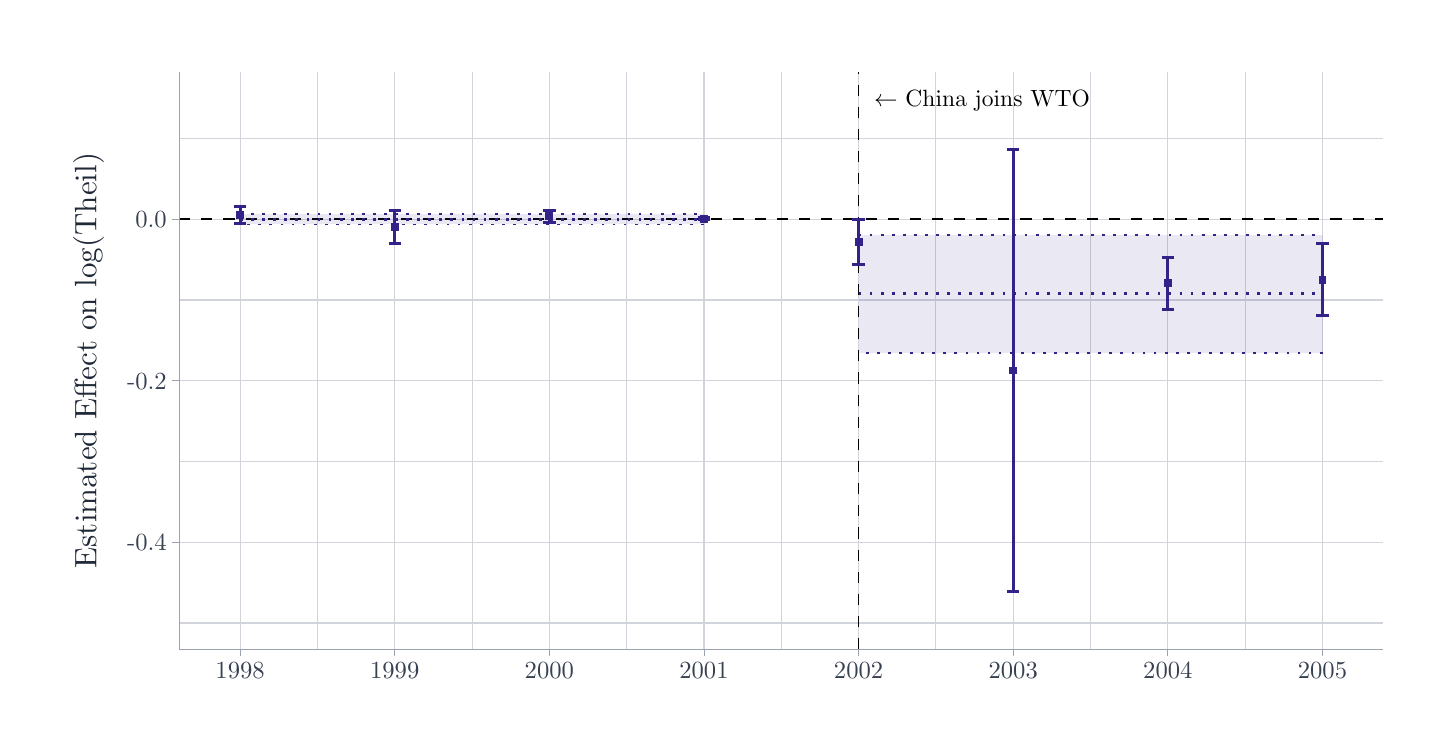
\begin{tikzpicture}[x=1pt,y=1pt]
\definecolor{fillColor}{RGB}{255,255,255}
\path[use as bounding box,fill=fillColor] (0,0) rectangle (505.89,252.94);
\begin{scope}
\path[clip] (  0.00,  0.00) rectangle (505.89,252.94);
\definecolor{drawColor}{RGB}{255,255,255}

\path[draw=drawColor,line width= 0.5pt,line join=round,line cap=round,fill=fillColor] (  0.00,  0.00) rectangle (505.89,252.94);
\end{scope}
\begin{scope}
\path[clip] ( 54.75, 28.35) rectangle (489.89,236.94);
\definecolor{drawColor}{RGB}{255,255,255}
\definecolor{fillColor}{RGB}{255,255,255}

\path[draw=drawColor,line width= 0.5pt,line join=round,line cap=round,fill=fillColor] ( 54.75, 28.35) rectangle (489.89,236.94);
\definecolor{drawColor}{RGB}{209,213,219}

\path[draw=drawColor,line width= 0.4pt,line join=round] ( 54.75, 37.83) --
	(489.89, 37.83);

\path[draw=drawColor,line width= 0.4pt,line join=round] ( 54.75, 96.18) --
	(489.89, 96.18);

\path[draw=drawColor,line width= 0.4pt,line join=round] ( 54.75,154.53) --
	(489.89,154.53);

\path[draw=drawColor,line width= 0.4pt,line join=round] ( 54.75,212.88) --
	(489.89,212.88);

\path[draw=drawColor,line width= 0.4pt,line join=round] (104.70, 28.35) --
	(104.70,236.94);

\path[draw=drawColor,line width= 0.4pt,line join=round] (160.58, 28.35) --
	(160.58,236.94);

\path[draw=drawColor,line width= 0.4pt,line join=round] (216.45, 28.35) --
	(216.45,236.94);

\path[draw=drawColor,line width= 0.4pt,line join=round] (272.32, 28.35) --
	(272.32,236.94);

\path[draw=drawColor,line width= 0.4pt,line join=round] (328.19, 28.35) --
	(328.19,236.94);

\path[draw=drawColor,line width= 0.4pt,line join=round] (384.07, 28.35) --
	(384.07,236.94);

\path[draw=drawColor,line width= 0.4pt,line join=round] (439.94, 28.35) --
	(439.94,236.94);

\path[draw=drawColor,line width= 0.4pt,line join=round] ( 54.75, 67.01) --
	(489.89, 67.01);

\path[draw=drawColor,line width= 0.4pt,line join=round] ( 54.75,125.35) --
	(489.89,125.35);

\path[draw=drawColor,line width= 0.4pt,line join=round] ( 54.75,183.70) --
	(489.89,183.70);

\path[draw=drawColor,line width= 0.4pt,line join=round] ( 76.77, 28.35) --
	( 76.77,236.94);

\path[draw=drawColor,line width= 0.4pt,line join=round] (132.64, 28.35) --
	(132.64,236.94);

\path[draw=drawColor,line width= 0.4pt,line join=round] (188.51, 28.35) --
	(188.51,236.94);

\path[draw=drawColor,line width= 0.4pt,line join=round] (244.38, 28.35) --
	(244.38,236.94);

\path[draw=drawColor,line width= 0.4pt,line join=round] (300.26, 28.35) --
	(300.26,236.94);

\path[draw=drawColor,line width= 0.4pt,line join=round] (356.13, 28.35) --
	(356.13,236.94);

\path[draw=drawColor,line width= 0.4pt,line join=round] (412.00, 28.35) --
	(412.00,236.94);

\path[draw=drawColor,line width= 0.4pt,line join=round] (467.88, 28.35) --
	(467.88,236.94);
\definecolor{drawColor}{RGB}{0,0,0}

\path[draw=drawColor,line width= 0.6pt,dash pattern=on 4pt off 4pt ,line join=round] ( 54.75,183.70) -- (489.89,183.70);

\path[draw=drawColor,line width= 0.6pt,dash pattern=on 4pt off 4pt ,line join=round] (300.26, 28.35) -- (300.26,236.94);

\node[text=drawColor,anchor=base west,inner sep=0pt, outer sep=0pt, scale=  0.85] at (305.85,224.52) {$\leftarrow$ China joins WTO};
\definecolor{drawColor}{RGB}{51,34,136}

\path[draw=drawColor,line width= 1.1pt,line join=round] ( 74.53,188.44) --
	( 79.00,188.44);

\path[draw=drawColor,line width= 1.1pt,line join=round] ( 76.77,188.44) --
	( 76.77,182.06);

\path[draw=drawColor,line width= 1.1pt,line join=round] ( 74.53,182.06) --
	( 79.00,182.06);

\path[draw=drawColor,line width= 1.1pt,line join=round] (130.40,186.72) --
	(134.87,186.72);

\path[draw=drawColor,line width= 1.1pt,line join=round] (132.64,186.72) --
	(132.64,175.10);

\path[draw=drawColor,line width= 1.1pt,line join=round] (130.40,175.10) --
	(134.87,175.10);

\path[draw=drawColor,line width= 1.1pt,line join=round] (186.28,186.93) --
	(190.75,186.93);

\path[draw=drawColor,line width= 1.1pt,line join=round] (188.51,186.93) --
	(188.51,182.55);

\path[draw=drawColor,line width= 1.1pt,line join=round] (186.28,182.55) --
	(190.75,182.55);

\path[draw=drawColor,line width= 1.1pt,line join=round] (242.15,184.34) --
	(246.62,184.34);

\path[draw=drawColor,line width= 1.1pt,line join=round] (244.38,184.34) --
	(244.38,183.49);

\path[draw=drawColor,line width= 1.1pt,line join=round] (242.15,183.49) --
	(246.62,183.49);

\path[draw=drawColor,line width= 1.1pt,line join=round] (298.02,183.71) --
	(302.49,183.71);

\path[draw=drawColor,line width= 1.1pt,line join=round] (300.26,183.71) --
	(300.26,167.32);

\path[draw=drawColor,line width= 1.1pt,line join=round] (298.02,167.32) --
	(302.49,167.32);

\path[draw=drawColor,line width= 1.1pt,line join=round] (353.90,209.06) --
	(358.37,209.06);

\path[draw=drawColor,line width= 1.1pt,line join=round] (356.13,209.06) --
	(356.13, 49.03);

\path[draw=drawColor,line width= 1.1pt,line join=round] (353.90, 49.03) --
	(358.37, 49.03);

\path[draw=drawColor,line width= 1.1pt,line join=round] (409.77,169.87) --
	(414.24,169.87);

\path[draw=drawColor,line width= 1.1pt,line join=round] (412.00,169.87) --
	(412.00,151.22);

\path[draw=drawColor,line width= 1.1pt,line join=round] (409.77,151.22) --
	(414.24,151.22);

\path[draw=drawColor,line width= 1.1pt,line join=round] (465.64,174.90) --
	(470.11,174.90);

\path[draw=drawColor,line width= 1.1pt,line join=round] (467.88,174.90) --
	(467.88,148.83);

\path[draw=drawColor,line width= 1.1pt,line join=round] (465.64,148.83) --
	(470.11,148.83);
\definecolor{fillColor}{RGB}{51,34,136}

\path[fill=fillColor] ( 75.34,183.82) --
	( 78.19,183.82) --
	( 78.19,186.67) --
	( 75.34,186.67) --
	cycle;

\path[fill=fillColor] (131.21,179.48) --
	(134.07,179.48) --
	(134.07,182.34) --
	(131.21,182.34) --
	cycle;

\path[fill=fillColor] (187.09,183.31) --
	(189.94,183.31) --
	(189.94,186.17) --
	(187.09,186.17) --
	cycle;

\path[fill=fillColor] (242.96,182.49) --
	(245.81,182.49) --
	(245.81,185.34) --
	(242.96,185.34) --
	cycle;

\path[fill=fillColor] (298.83,174.09) --
	(301.68,174.09) --
	(301.68,176.94) --
	(298.83,176.94) --
	cycle;

\path[fill=fillColor] (354.70,127.62) --
	(357.56,127.62) --
	(357.56,130.47) --
	(354.70,130.47) --
	cycle;

\path[fill=fillColor] (410.58,159.12) --
	(413.43,159.12) --
	(413.43,161.97) --
	(410.58,161.97) --
	cycle;

\path[fill=fillColor] (466.45,160.44) --
	(469.30,160.44) --
	(469.30,163.29) --
	(466.45,163.29) --
	cycle;
\definecolor{fillColor}{RGB}{51,34,136}

\path[fill=fillColor,fill opacity=0.10] (300.26,178.11) --
	(467.88,178.11) --
	(467.88,135.38) --
	(300.26,135.38) --
	cycle;

\path[draw=drawColor,line width= 0.6pt,dash pattern=on 1pt off 3pt ,line join=round] (300.26,178.11) --
	(467.88,178.11);

\path[draw=drawColor,line width= 0.6pt,dash pattern=on 1pt off 3pt ,line join=round] (467.88,135.38) --
	(300.26,135.38);

\path[fill=fillColor,fill opacity=0.10] ( 76.77,185.55) --
	(244.38,185.55) --
	(244.38,181.85) --
	( 76.77,181.85) --
	cycle;

\path[draw=drawColor,line width= 0.6pt,dash pattern=on 1pt off 3pt ,line join=round] ( 76.77,185.55) --
	(244.38,185.55);

\path[draw=drawColor,line width= 0.6pt,dash pattern=on 1pt off 3pt ,line join=round] (244.38,181.85) --
	( 76.77,181.85);

\path[draw=drawColor,line width= 1.1pt,dash pattern=on 1pt off 3pt ,line join=round] (300.26,156.74) --
	(467.88,156.74);

\path[draw=drawColor,line width= 1.1pt,dash pattern=on 1pt off 3pt ,line join=round] ( 76.77,183.70) --
	(244.38,183.70);
\end{scope}
\begin{scope}
\path[clip] (  0.00,  0.00) rectangle (505.89,252.94);
\definecolor{drawColor}{RGB}{156,163,175}

\path[draw=drawColor,line width= 0.3pt,line join=round] ( 54.75, 28.35) --
	( 54.75,236.94);
\end{scope}
\begin{scope}
\path[clip] (  0.00,  0.00) rectangle (505.89,252.94);
\definecolor{drawColor}{RGB}{55,65,81}

\node[text=drawColor,anchor=base east,inner sep=0pt, outer sep=0pt, scale=  0.89] at ( 50.25, 63.94) {-0.4};

\node[text=drawColor,anchor=base east,inner sep=0pt, outer sep=0pt, scale=  0.89] at ( 50.25,122.29) {-0.2};

\node[text=drawColor,anchor=base east,inner sep=0pt, outer sep=0pt, scale=  0.89] at ( 50.25,180.64) {0.0};
\end{scope}
\begin{scope}
\path[clip] (  0.00,  0.00) rectangle (505.89,252.94);
\definecolor{drawColor}{RGB}{156,163,175}

\path[draw=drawColor,line width= 0.3pt,line join=round] ( 52.25, 67.01) --
	( 54.75, 67.01);

\path[draw=drawColor,line width= 0.3pt,line join=round] ( 52.25,125.35) --
	( 54.75,125.35);

\path[draw=drawColor,line width= 0.3pt,line join=round] ( 52.25,183.70) --
	( 54.75,183.70);
\end{scope}
\begin{scope}
\path[clip] (  0.00,  0.00) rectangle (505.89,252.94);
\definecolor{drawColor}{RGB}{156,163,175}

\path[draw=drawColor,line width= 0.3pt,line join=round] ( 54.75, 28.35) --
	(489.89, 28.35);
\end{scope}
\begin{scope}
\path[clip] (  0.00,  0.00) rectangle (505.89,252.94);
\definecolor{drawColor}{RGB}{156,163,175}

\path[draw=drawColor,line width= 0.3pt,line join=round] ( 76.77, 25.85) --
	( 76.77, 28.35);

\path[draw=drawColor,line width= 0.3pt,line join=round] (132.64, 25.85) --
	(132.64, 28.35);

\path[draw=drawColor,line width= 0.3pt,line join=round] (188.51, 25.85) --
	(188.51, 28.35);

\path[draw=drawColor,line width= 0.3pt,line join=round] (244.38, 25.85) --
	(244.38, 28.35);

\path[draw=drawColor,line width= 0.3pt,line join=round] (300.26, 25.85) --
	(300.26, 28.35);

\path[draw=drawColor,line width= 0.3pt,line join=round] (356.13, 25.85) --
	(356.13, 28.35);

\path[draw=drawColor,line width= 0.3pt,line join=round] (412.00, 25.85) --
	(412.00, 28.35);

\path[draw=drawColor,line width= 0.3pt,line join=round] (467.88, 25.85) --
	(467.88, 28.35);
\end{scope}
\begin{scope}
\path[clip] (  0.00,  0.00) rectangle (505.89,252.94);
\definecolor{drawColor}{RGB}{55,65,81}

\node[text=drawColor,anchor=base,inner sep=0pt, outer sep=0pt, scale=  0.89] at ( 76.77, 17.73) {1998};

\node[text=drawColor,anchor=base,inner sep=0pt, outer sep=0pt, scale=  0.89] at (132.64, 17.73) {1999};

\node[text=drawColor,anchor=base,inner sep=0pt, outer sep=0pt, scale=  0.89] at (188.51, 17.73) {2000};

\node[text=drawColor,anchor=base,inner sep=0pt, outer sep=0pt, scale=  0.89] at (244.38, 17.73) {2001};

\node[text=drawColor,anchor=base,inner sep=0pt, outer sep=0pt, scale=  0.89] at (300.26, 17.73) {2002};

\node[text=drawColor,anchor=base,inner sep=0pt, outer sep=0pt, scale=  0.89] at (356.13, 17.73) {2003};

\node[text=drawColor,anchor=base,inner sep=0pt, outer sep=0pt, scale=  0.89] at (412.00, 17.73) {2004};

\node[text=drawColor,anchor=base,inner sep=0pt, outer sep=0pt, scale=  0.89] at (467.88, 17.73) {2005};
\end{scope}
\begin{scope}
\path[clip] (  0.00,  0.00) rectangle (505.89,252.94);
\definecolor{drawColor}{RGB}{31,41,55}

\node[text=drawColor,rotate= 90.00,anchor=base,inner sep=0pt, outer sep=0pt, scale=  1.12] at ( 24.84,132.65) {Estimated Effect on $\log($Theil$)$};
\end{scope}
\end{tikzpicture}
